\documentclass[10pt]{article}
\usepackage[utf8]{inputenc}
\usepackage[includehead, headheight=10mm, margin=15mm ]{geometry}
\usepackage{amsmath}
\usepackage{amsthm}
\usepackage{amsfonts}
\usepackage{xcolor}
\usepackage{graphicx}
\usepackage{titling}
\usepackage{fancyhdr}
\usepackage{listings}
\usepackage{hyperref}

\title{APPM 4600 Lab 12}
\author{Edward Wawrzynek}
\date{14 November 2024}

\newcommand*{\dif}{\mathop{}\!\mathrm{d}}

\makeatletter
\def\@maketitle{%
  \newpage
  \null
  \vskip 1em%
  \begin{center}%
  \let \footnote \thanks
    {\LARGE \@title \par}%
    \vskip 1em%
    {\normalfont \@date}
  \end{center}%
  \par
  \vskip 1em}
\makeatother

\begin{document}

\pagestyle{fancy}
    \fancyhf{} % clear all header and footer fields
    \fancyhead[L]{\thetitle}
    \fancyhead[R]{\theauthor}

\makeatletter
\begin{center}
    {\Large \@title}
    \vskip 1mm
    {\normalfont \@date}
    \vskip 1em
\end{center}
\makeatother

The code for this lab can be seen at the end of this document, or on github \href{https://github.com/edwardwawrzynek/APPM4600/blob/master/Labs/Lab\%2012}{here}.

\section{Prelab}
\begin{enumerate}
  \item The code to evaluate composite trapezoidal and simpsons is included in the attached code, in the functions \texttt{eval\_composite\_trap} and \texttt{eval\_composite\_simpsons}.
\end{enumerate}

\section{Adaptive Quadrature}

We use adaptive quadrature to evaluate the integral \begin{align*}
    I = \int_{0.1}^{2} \sin  \left( \frac{1}{x} \right) \dif x,
\end{align*} with \(n=5\) nodes on each interval. 

Gauss quadrature requires 6 intervals (5 splits) to get to the desired accuracy. The absolute accuracy versus \(n\) and final evaluation points for \(n=5\) are plotted below.

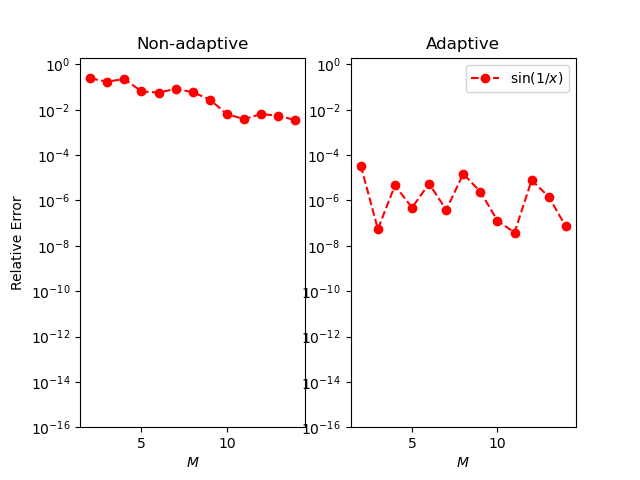
\includegraphics[width=0.45\textwidth]{gauss.png}
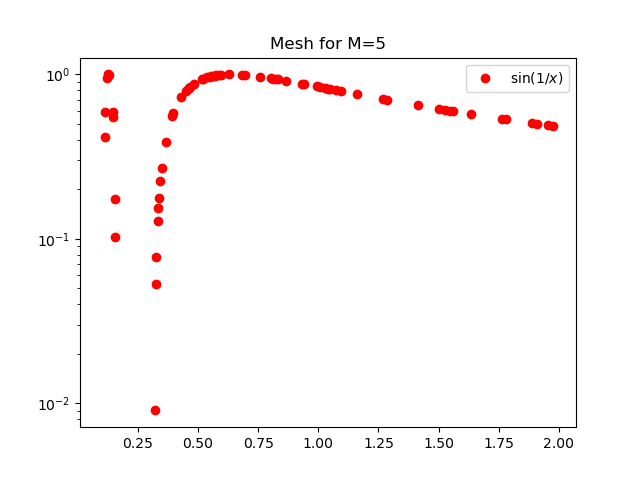
\includegraphics[width=0.45\textwidth]{gauss_mesh.png}

Composite trapezoidal requires 9 intervals (8 splits) to get to the desired accuracy. The absolute accuracy versus \(n\) and final evaluation points for \(n=5\) are plotted below.

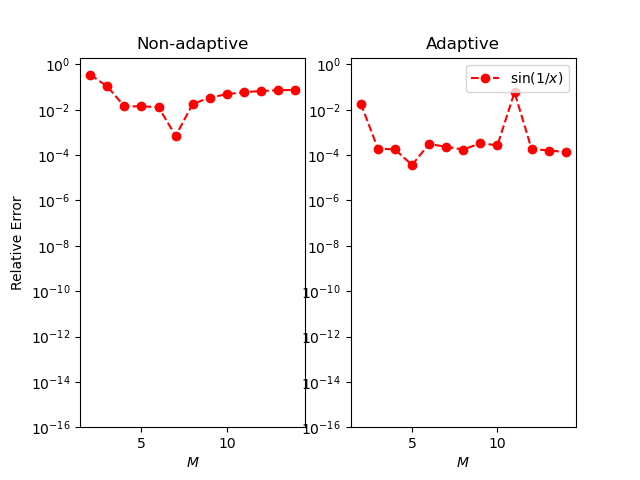
\includegraphics[width=0.45\textwidth]{trap.png}
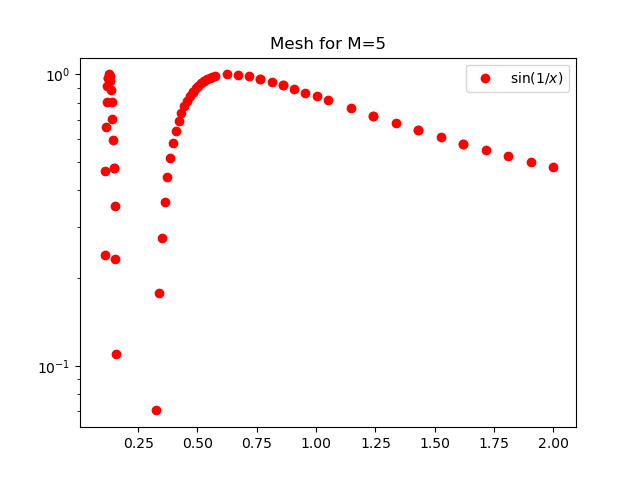
\includegraphics[width=0.45\textwidth]{trap_mesh.png}

Composite Simpsons requires 6 intervals (5 splits) to get to the desired accuracy. The absolute accuracy versus \(n\) and final evaluation points for \(n=5\) are plotted below.

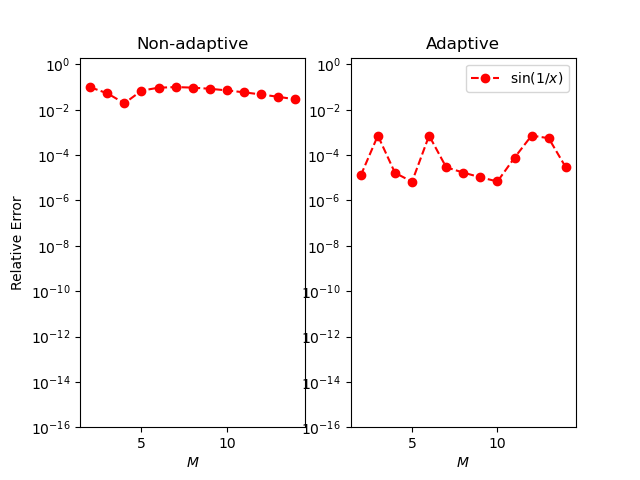
\includegraphics[width=0.45\textwidth]{simp.png}
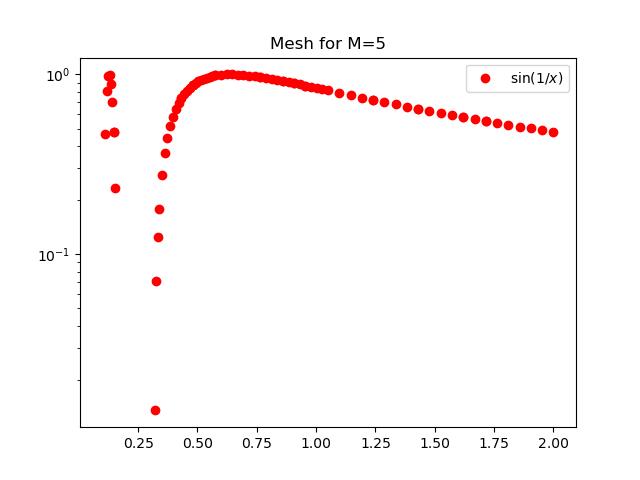
\includegraphics[width=0.45\textwidth]{simp_mesh.png}

{\small \lstinputlisting[language=Python]{adaptive_quad.py}}
{\small \lstinputlisting[language=Python]{adaptive_quad_test.py}}    

\end{document}
